%%%%%%%%%%%%%
%% METHODS %%
%%%%%%%%%%%%%

%This chapter describes in detail the methods for whatever activities were necessary for your project – e.g., data gathering, data analysis, requirements analysis, design, implementation, testing/evaluation, etc. Your choice of methods should be discussed and justified in view of the project objectives, and with reference to the pertinent literature. Report not only what methods you applied in generic terms, but what you actually did: sufficient information about dates and details for your reader to understand how you ran your project, rather than just how one could run any similar project. 

\chapter{Methods}
\label{Methods} 

\section{Simulators}

In this section we examine some simulators currently available to the task of training autonomous systems, to the be able to consider safety aspects of such models.

\subsection{AirSim}

The AirSim \cite{airsim2017fsr} is a simulator for autonomous vehicles, aimed to be a platform for AI research.

The paper was accepted for the Field and Service Robotics 10th International Conference. No other papers seam to deal with simulators, at least in the title. AirSim references 23 articles.

\subsection{Applying Noise to Images}

\subsection{Carla}

\subsection{weight initialisation}

\subsection{MNIST Dataset}

The MNIST dataset, a cornerstone in the field of machine learning, serves as a benchmark for evaluating the performance of algorithms in the domain of handwritten digit recognition. Comprising a collection of 70,000 grayscale images, each of 28x28 pixel resolution, the dataset is divided into two distinct sets: a training set containing 60,000 examples, and a test set with 10,000 examples (\cite{LeCun1998}). Each image within the dataset is associated with a label from 0 to 9, corresponding to the digit it represents.

This dataset has been instrumental in facilitating advancements in machine learning, particularly in the development and evaluation of algorithms capable of performing classification tasks. Its widespread adoption can be attributed to several factors, including the simplicity of the task it presents and its suitability for use in benchmarking the performance of various learning algorithms, ranging from simple linear classifiers to more complex deep learning models.

A key feature of the MNIST dataset is its pre-processing stage, where the digits have been size-normalized and centered in a fixed-size image. This pre-processing reduces the variability unrelated to digit identity, allowing researchers to focus on the algorithmic challenge of digit recognition rather than on the preprocessing steps.

The significance of the MNIST dataset in the realm of machine learning research is well-documented, with \cite{LeCun1998} providing an extensive overview of the dataset's creation, characteristics, and its role in fostering advancements in the field.

This foundational dataset has not only enabled the comparison of algorithmic performance in a standardized setting but has also contributed to the proliferation of research in neural networks, serving as a pivotal benchmark for innovations in the field.

% Dataset description

The MNIST dataset is comprised of two main components: image files and label files, structured as follows:

\begin{itemize}
    \item \textbf{Training Set Images:} Contains 60,000 training examples.
    \item \textbf{Test Set Images:} Contains 10,000 test examples.
    \item Each image is encoded as a 28x28 pixel grid, summing up to 784 pixels per image. Each pixel represents a grayscale intensity, with 0 indicating white and 255 denoting black.
\end{itemize}

The structure of the image files is detailed below:
\begin{enumerate}
    \item \textbf{Magic Number:} The first 4 bytes signify a magic number (2051) that identifies the file format.
    \item \textbf{Number of Images:} The following 4 bytes denote the count of images, encoded as a 32-bit integer.
    \item \textbf{Rows:} The subsequent 4 bytes illustrate the number of rows (28) per image, encoded as a 32-bit integer.
    \item \textbf{Columns:} The next 4 bytes depict the number of columns (28) per image, encoded as a 32-bit integer.
    \item \textbf{Pixel Values:} The remainder of the file is populated with pixel values in row-major order, with each image delineated sequentially in the file. Each pixel value is stored as an unsigned byte, representing the pixel's intensity.
\end{enumerate}

and label files:
\begin{itemize}
    \item \textbf{Training Set Labels:} Comprises 60,000 labels corresponding to the training images.
    \item \textbf{Test Set Labels:} Comprises 10,000 labels corresponding to the test images.
    \item Each label is a single byte signifying the digit (0 through 9) that the corresponding image represents.
\end{itemize}

The structure of the label files is detailed below:
\begin{enumerate}
    \item \textbf{Magic Number:} The first 4 bytes signify a magic number (2049) that identifies the file format.
    \item \textbf{Number of Items:} The following 4 bytes denote the count of labels, encoded as a 32-bit integer.
    \item \textbf{Labels:} The remainder of the file contains label values, stored as unsigned bytes, with each label corresponding to the image of the same index in the image file.
\end{enumerate}

This standardized format ensures the MNIST dataset's compatibility with a wide array of machine learning models, particularly facilitating research in image classification and handwriting recognition.

\begin{table}[h]
\centering
\begin{tabular}{|l|l|r|r|}
\hline
\textbf{Type}             & \textbf{File Name}                       & \textbf{Size (B)} & \textbf{Count} \\ \hline
Training Images & \texttt{train-images-idx3-ubyte} & 47040016           & 60000 \\
Training Labels & \texttt{train-labels-idx1-ubyte} & 60008             & 60000 \\
Testing Images  & \texttt{t10k-images-idx3-ubyte}  & 7840016           & 10000 \\
Testing Labels  & \texttt{t10k-labels-idx1-ubyte}  & 10008              & 10000 \\ \hline
\end{tabular}
\caption{MNIST Dataset Files, file sizes in bytes and image/label count}
\label{table:mnist_files_b}
\end{table}
The contents can be examined with the \textit{xxd} command:
\begin{verbatim}
!xxd -C 'data/MNIST/raw/train-images-idx3-ubyte' | head

00000000: 0000 0803 0000 ea60 0000 001c 0000 001c  .......`........
00000010: 0000 0000 0000 0000 0000 0000 0000 0000  ................
00000020: 0000 0000 0000 0000 0000 0000 0000 0000  ................
00000030: 0000 0000 0000 0000 0000 0000 0000 0000  ................
00000040: 0000 0000 0000 0000 0000 0000 0000 0000  ................
00000050: 0000 0000 0000 0000 0000 0000 0000 0000  ................
00000060: 0000 0000 0000 0000 0000 0000 0000 0000  ................
00000070: 0000 0000 0000 0000 0000 0000 0000 0000  ................
00000080: 0000 0000 0000 0000 0000 0000 0000 0000  ................
00000090: 0000 0000 0000 0000 0000 0000 0000 0000  ................

!xxd -C 'data/MNIST/raw/train-labels-idx1-ubyte' | head

00000000: 0000 0801 0000 ea60 0500 0401 0902 0103  .......`........
00000010: 0104 0305 0306 0107 0208 0609 0400 0901  ................
00000020: 0102 0403 0207 0308 0609 0005 0600 0706  ................
00000030: 0108 0709 0309 0805 0903 0300 0704 0908  ................
00000040: 0009 0401 0404 0600 0405 0601 0000 0107  ................
00000050: 0106 0300 0201 0107 0900 0206 0708 0309  ................
00000060: 0004 0607 0406 0800 0708 0301 0507 0107  ................
00000070: 0101 0603 0002 0903 0101 0004 0902 0000  ................
00000080: 0200 0207 0108 0604 0106 0304 0509 0103  ................
00000090: 0308 0504 0707 0402 0805 0806 0703 0406  ................
\end{verbatim}
Where hex \textbf{0000 0803} is the magic number 2051 (images), and hex \textbf{0000 0801} is the magic number 2049 (labels), hex \textbf{0000 ea60}, 60,000 decimal, is the number of examples in the dataset, and hex \textbf{0000 001c}, decimal 28, is the number of rows, and columns, in every image. Therefore the number of bytes in train-images-idx3-ubyte is $4 * 4 + 60000 * 28 * 28 = 47,040,016$.

The first image in the training dataset can be obtained by offsetting the first 16 bytes (magic number, number of images, row size and column size) and taking the next 784 bytes, then splitting the array into 28 rows.


\begin{figure}[h]
    \centering
    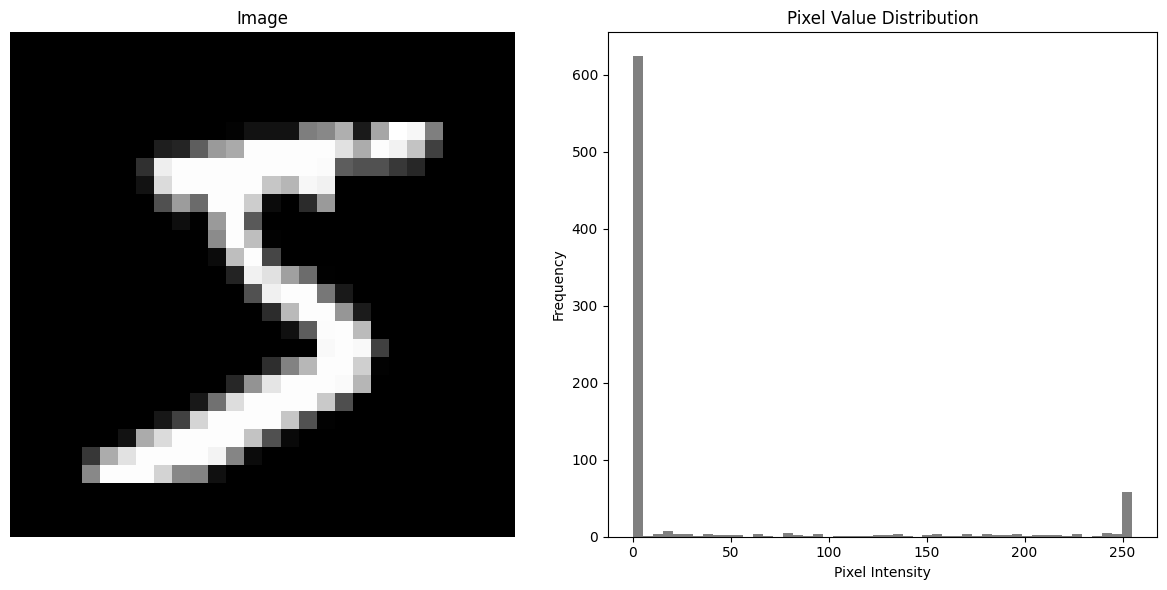
\includegraphics[width=0.75\textwidth]{Figures/Methods/MNIST_5_with_histogram.png}
    \caption{MNIST digit 5 and its pixel value distribution histogram.}
    \label{fig:mnist_5_histogram}
\end{figure}
As shown in Figure~\ref{fig:mnist_5_histogram}, the MNIST digit 5 is displayed alongside its pixel value distribution histogram where the pixel values range from 0 to 255. Figure~\ref{fig:mnist_0_histogram} shows the second image (zero) in the MNIST training dataset.

\begin{figure}[h]
    \centering
    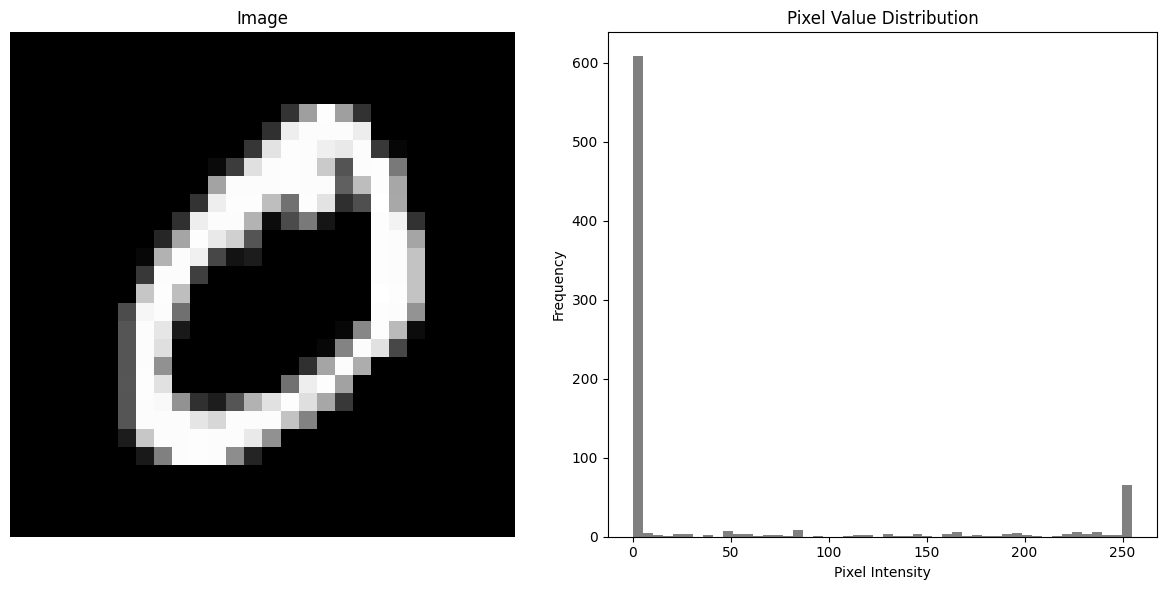
\includegraphics[width=0.75\textwidth]{Figures/Methods/MNIST_0_with_histogram.png}
    \caption{MNIST digit 0 and its pixel value distribution histogram.}
    \label{fig:mnist_0_histogram}
\end{figure}

From the training labels dataset, it can be seen that by offsetting the magic number and the number of labels, represented by 4 bytes each, the following bytes represent the labels, that is, the first two labels are "05 and "00", matching figures \ref{fig:mnist_5_histogram} and \ref{fig:mnist_0_histogram}.

\subsection{Creating the "noisy" MNIST dataset}

To augment the research on image recognition robustness, we propose the creation of an enhanced training and testing dataset derived from the original MNIST dataset. This new dataset will incorporate a variety of perturbations to the original images, aiming to simulate real-world conditions where image data may not be ideal. Specifically, we will introduce noise to the images using 12 distinct functions designed to add perturbations, categorized as follows:

\begin{enumerate}
    \item \textbf{Pixel Intensity Adjustment:}
    \begin{itemize}
        \item Brightness
        \item Contrast
    \end{itemize}
    \item \textbf{Blurring:}
    \begin{itemize}
        \item Defocus Blur
        \item Motion Blur
        \item Zoom Blur
    \end{itemize}
    \item \textbf{Noise:}
    \begin{itemize}
        \item Gaussian Noise
        \item Impulse Noise
        \item Shot Noise
    \end{itemize}
    \item \textbf{Weather:}
    \begin{itemize}
        \item Fog
        \item Frost
        \item Snow
    \end{itemize}
    \item \textbf{Special Effects:}
    \begin{itemize}
        \item Pixelation
    \end{itemize}
\end{enumerate}

Each image in the original dataset will undergo transformation by one or more of these perturbation methods, resulting in a companion image that retains the original label but exhibits the added noise or effect. The resultant dataset will consist of pairs of images: the clean (original) and the noisy (perturbed) versions. To facilitate distinction and subsequent analysis, labels will be appended to denote the image type: "00" for clean/original images and "01" for noisy/perturbed images. This dual dataset structure will enable comprehensive evaluation of machine learning models' performance in recognizing digits under varied conditions, thereby enhancing the robustness of image recognition technologies.

% Applying noise

To generate our new dataset, we write to a binary file named perturbed-train-images-idx3-ubyte, where the first 16 bytes are:
\begin{verbatim}
0000 0803 0001 d4c0 0000 001c 0000 001c    
\end{verbatim}
Where 0001 d4c0 hex is 120000 decimal, the size of the new training dataset, twice the size of the original dataset.

We make a random selection of a perturbation type, and a perturbation level ranging from 0 to 9, and apply the perturbation to the image.

Figures \ref{fig:MNIST_4_clean_with_histogram} and \ref{fig:MNIST_4_noisy_with_histogram} show digit 4 with no noise and zoom blur level 8 applied.
\begin{figure}[h]
    \centering
    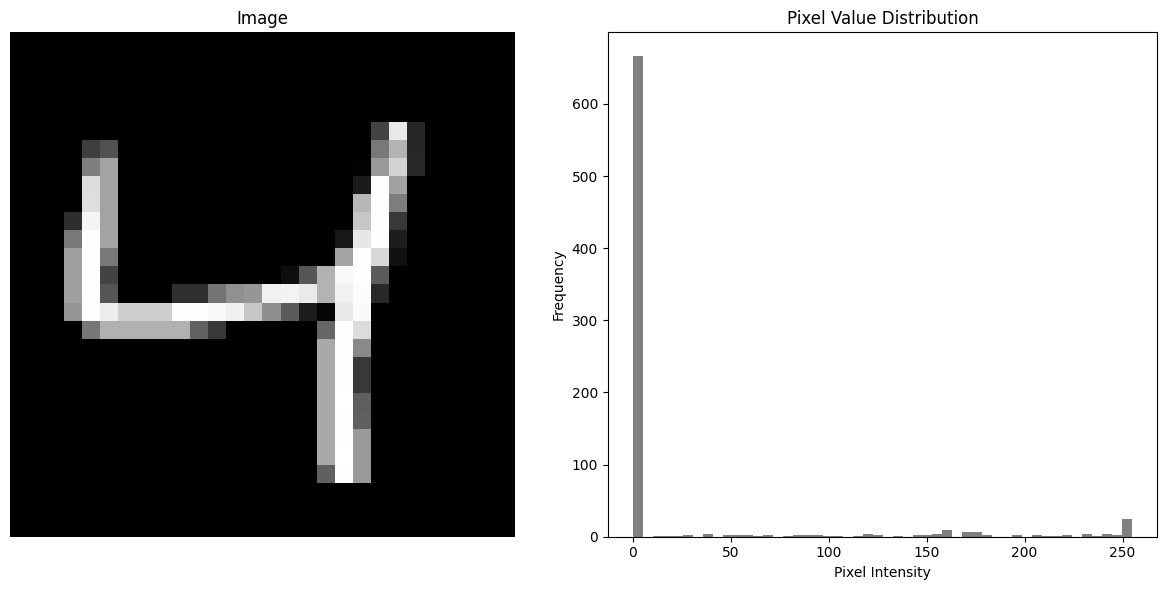
\includegraphics[width=0.75\textwidth]{Figures/Methods/MNIST_4_clean_with_histogram.png}
    \caption{MNIST digit 4 with no noise.}
    \label{fig:MNIST_4_clean_with_histogram}
\end{figure}

\begin{figure}[h]
    \centering
    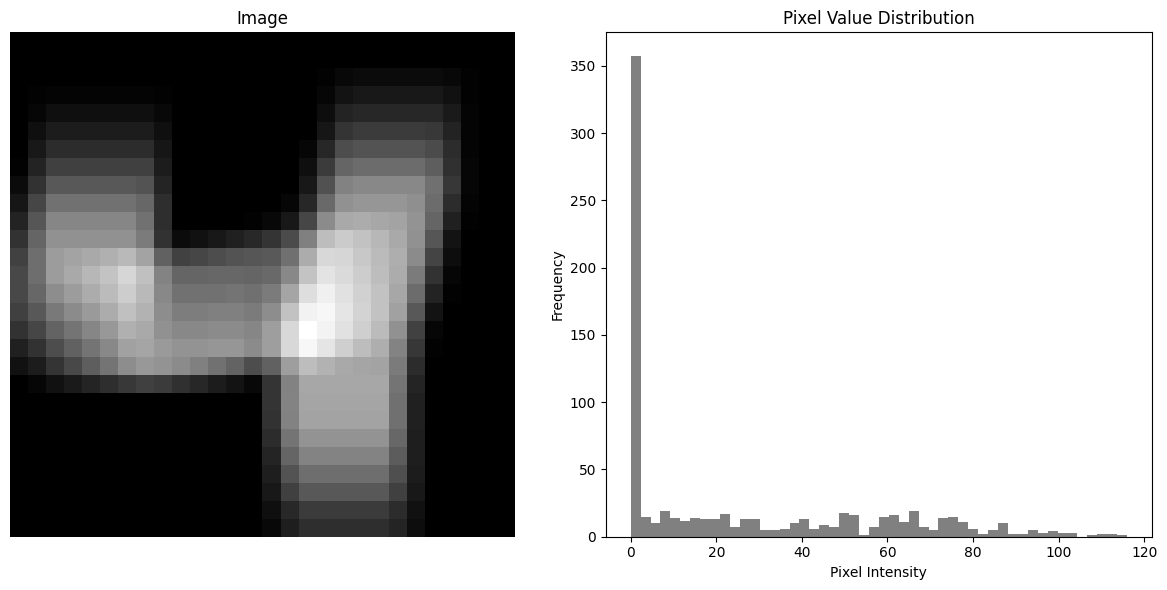
\includegraphics[width=0.75\textwidth]{Figures/Methods/MNIST_4_noisy_with_histogram.png}
    \caption{MNIST digit 4 with Zoom Blur level 8.}
    \label{fig:MNIST_4_noisy_with_histogram}
\end{figure}

% file to generate images is
% https://colab.research.google.com/drive/1s-KBSwUtT7tp280iLi8KgyHk4zThDnKD#scrollTo=OMq-a-wuKqR0
% MNIST-Dataset.ipynb

The process can be describe like so:

\begin{lstlisting}[caption={MNIST Perturbation Algorithm}, label={lst:mnist_perturbation_algorithm}]
Function createFiles():
    Open images.bin as binary write
    Open labels.bin as binary write
    Open perturbations.bin as binary write

Function saveImage(image, file):
    Write image to file

Function saveLabel(label, file):
    Write label to file as a single byte

Function savePerturbation(perturbationCode, file):
    Write perturbationCode to file as bytes

Function main():
    createFiles()
    For each image in MNIST:
        saveImage(originalImage, images.bin)
        saveLabel(0x00, labels.bin)
        savePerturbation(0xFFFF, perturbations.bin)
        
        perturbedImage = applyRandomPerturbation(originalImage)
        saveImage(perturbedImage, images.bin)
        saveLabel(0x01, labels.bin)
        perturbationCode = getPerturbationCode()
        savePerturbation(perturbationCode, perturbations.bin)

\end{lstlisting}

We apply the same process to training and testing datasets, and end up with 6 files as shown in Table \ref{table:mnist_perturbed_files_b}.

% \begin{table}[h]
% \centering
% \begin{tabular}{|l|l|r|r|}
% \hline
% \textbf{Type}             & \textbf{File Name}                          & \textbf{Size (B)} & \textbf{Count} \\ \hline
% Perturbed Training Images  & \texttt{perturbed-train-images-idx3-ubyte}    & TBA               & 120000 \\                            
% Perturbed Training Labels  & \texttt{perturbed-train-labels-idx1-ubyte}    & TBA               & 120000 \\                            
% Perturbation Training Levels  & \texttt{perturbation-train-levels-idx0-ubyte} & TBA               & 120000 \\
% Perturbed Testing Images   & \texttt{t20k-perturbed-images-idx3-ubyte}     & TBA               & 20000 \\                            
% Perturbed Testing Labels   & \texttt{t20k-perturbed-labels-idx1-ubyte}     & TBA               & 20000 \\  
% Perturbation Testing Levels   & \texttt{t20k-perturbation-levels-idx0-ubyte}     & TBA               & 20000 \\ \hline                 
% \end{tabular}
% \caption{Perturbed MNIST (PMNIST) Dataset Files, file sizes in bytes and image/label count}
% \label{table:mnist_perturbed_files_b}
% \end{table}

\begin{table}[h]
\centering
{\small
\begin{tabular}{|l|l|l|r|r|}
\hline
\textbf{ID} & \textbf{Type}                   & \textbf{File Name}                                   & \textbf{Size (B)} & \textbf{Count} \\ \hline
1 & Perturbed Training Images       & \texttt{perturbed-train-images-idx3-ubyte}    & TBA               & 120000 \\
2 & Perturbed Training Labels       & \texttt{perturbed-train-labels-idx1-ubyte}    & TBA               & 120000 \\
3 & Perturbation Training Levels    & \texttt{perturbation-train-levels-idx0-ubyte} & TBA               & 120000 \\
4 & Perturbed Testing Images        & \texttt{t20k-perturbed-images-idx3-ubyte}     & TBA               & 20000 \\
5 & Perturbed Testing Labels        & \texttt{t20k-perturbed-labels-idx1-ubyte}     & TBA               & 20000 \\
6 & Perturbation Testing Levels     & \texttt{t20k-perturbation-levels-idx0-ubyte}  & TBA               & 20000 \\ \hline
\end{tabular}
} % End of \small
\caption{Perturbed MNIST (PMNIST) Dataset Files, file sizes in bytes and image/label count}
\label{table:mnist_perturbed_files_b}
\end{table}

Where the additional files are perturbation-train-levels-idx0-ubyte and t20k-perturbation-levels-idx0-ubyte that contain the perturbation types and levels, stored contiguously in one byte values. As per the algorithm listed in Listing \ref{lst:mnist_perturbation_algorithm}, We start by opening the binary files. We then iterate over every image in the MNIST dataset. We apply a random perturbation and perturbation level to the image, writing the original and perturbed image to the new PMNIST dataset (ID 1). We write the image label twice (ID 2), once with value 0 indicating the image is noise-free, and once with value 1 indicating the image is perturbed, aligning with the saved images and finally we write the perturbation key and level (ID 3). We repeat the steps for the testing dataset, obtaining 3 additional files (IDs 4, 5 and 6).







